\newpage

    \begin{definition}{Common Notation}{14cm}
        The notes will be using common mathematical notations.

        \hspace{0.5cm}
        $\mathbb{Z}$
        \hspace{3cm}
        The set of all integers

        \hspace{0.5cm}
        $\mathbb{Q}$
        \hspace{3cm}
        The set of all rational numbers

        \hspace{0.5cm}
        $\mathbb{R}$
        \hspace{3cm}
        The set of all real numbers

        \hspace{0.5cm}
        $\mathbb{C}$
        \hspace{3cm}
        The set of all complex numbers

        \hspace{0.5cm}
        \{$x_1,...,x_n$\}
        \hspace{1.35cm}
        Finite set with elements $x_1,x_2,x_3,...,x_n$

        \hspace{0.5cm}
        x $\in$ E
        \hspace{2.3cm}
        x is an element of set E

        \hspace{0.5cm}
        x $\not \in$ E
        \hspace{2.3cm}
        x is not an element of set E

        \hspace{0.5cm}
        A $\subset$ B
        \hspace{2.2cm}
        Set A is a subset set E

        \hspace{0.5cm}
        A $\not \subset$ B
        \hspace{2.2cm}
        Set A is not a subset set E

        \hspace{0.5cm}
        f: A $\rightarrow$ B
        \hspace{1.7cm}
        Function f maps set A into set B

        To note, most theorems will include proofs, but some are
        beyond the scope of this course and thus, not included.
        However, none of the proofs are required in order for
        these theorems to be applied.
    \end{definition}



\section[Day 1: Vectors]{ Vectors }

\subsection{ Vectors }

    \begin{definition}{Vectors}{14cm}
        A {\color{lblue} scalar} c is a number in $\mathbb{R}$.

        A {\color{lblue} vector} x $\in$ $\mathbb{R}^n$
        is an ordered n-tuple of real numbers.

        \hspace{0.5cm}
        x = $(x_1,...,x_n)$ = $<x_1,...,x_n>$
        \hspace{1cm}
        where each $x_i$ $\in$ $\mathbb{R}$

        Let the zero vector 0 = (0,...,0).

        \vspace{0.3cm}

        If x,y $\in$ $\mathbb{R}^n$ and c is a scalar:

        \hspace{0.5cm}
        Comparison:
        \hspace{2.5cm}
        x = y if $x_i$ = $y_i$ for i = \{1,...,n\}

        \hspace{0.5cm}
        Vector Addition:
        \hspace{1.75cm}
        x+y = $(x_1+y_1,...,x_n+y_n)$

        \hspace{0.5cm}
        Scalar Multiplicaton:
        \hspace{1cm}
        cx = ($cx_1,...,cx_n$)
    \end{definition}

    \begin{figure}[h]
        \centering
        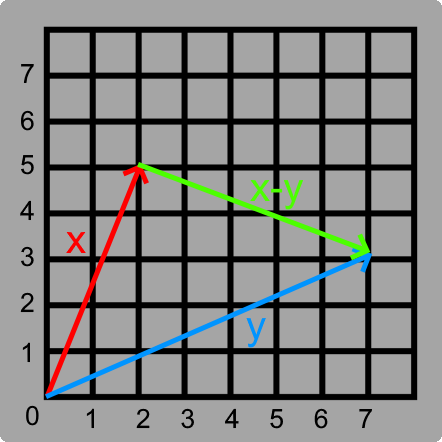
\includegraphics[scale=0.4]{Images/1.1.1.png}   
    \end{figure}



    \begin{ltheorem}{Vector Operations}{1.5cm}
        \item x+y = y+x
        
            \begin{proof}[14cm]
                x+y
                = $(x_1+y_1,...,x_n+y_n)$
                = $(y_1+x_1,...,y_n+x_n)$
                = y+x  
            \end{proof}

        \item x+(y+z) = (x+y)+z
            
            \begin{proof}[14cm]
                x+(y+z)
                = $(x_1,...,x_n)$ + $(y_1+z_1,...,y_n+z_n)$
                = $(x_1+y_1+z_1,...,x_n+y_n+z_n)$
                
                \hspace{1.6cm}
                = $(x_1+y_1,...,x_n+y_n)$ + $(z_1,...,z_n)$
                = (x+y)+z
            \end{proof}

            \newpage

        \item x+0 = x
            
            \begin{proof}[14cm]
                x+0
                = $(x_1+0,...,x_n+0)$
                = $(x_1,...,x_n)$
                = x
            \end{proof}

        \item c(x+y) = cx + cy
            
            \begin{proof}[14cm]
                c(x+y)
                = $(c(x_1+y_1),...,c(x_n+y_n))$
                = $(cx_1+cy_1,...,cx_n+cy_n)$
                = cx+cy
            \end{proof}

        \item (c+k)v = cv + kv
            
            \begin{proof}[14cm]
                (c+k)v
                = $((c+k)v_1,...,(c+k)v_n)$
                = $(cv_1+kv_1,...,cv_n+kv_n)$
                = cv+kv
            \end{proof}

        \item c(kx) = (ck)x = k(cx)
            
            \begin{proof}[14cm]
                c(kv)
                = $(c(kx_1),...,c(kx_n))$
                = $(ckx_1,...,ckx_n)$
                = (ck)x
                = $(kcx_1,...,kcx_n)$
                
                \hspace{1cm}
                = $(k(cx_1),...,k(cx_n))$
                = k(cx)
            \end{proof}
    \end{ltheorem}

    \vspace{0.5cm}



    \begin{definition}{Standard Basis Vectors}{14cm}
        The {\color{lblue} standard basis vectors} for $\mathbb{R}^n$
        are $e_1,...,e_n$ where each i = \{1,...,n\}:

        \hspace{0.5cm}
        $e_i$ = ($\underset{\scriptscriptstyle 1}{0},
                    \underset{\scriptscriptstyle 2}{0},...,
                    \underset{\scriptscriptstyle i-1}{0},
                    \underset{\scriptscriptstyle i}{1},
                    \underset{\scriptscriptstyle i+1}{0},...,
                    \underset{\scriptscriptstyle n-1}{0},
                    \underset{\scriptscriptstyle n}{0},$)

        Thus, for any x $\in$ $\mathbb{R}^n$:

        \hspace{0.5cm}
        x = $(x_1,...,x_n)$
        = $x_1e_1 + ... + x_ne_n$
    \end{definition}

    \vspace{0.5cm}



    \begin{example}
        Let x = (4,-2,5) and y = (-7,1,2). Find 3x-2y in standard basis vectors.
    \end{example}

    \begin{tbox}
        3x+y
        = $3\begin{bmatrix}
            4 \\
            -2 \\
            5
        \end{bmatrix} - 2
        \begin{bmatrix}
            -7 \\
            1 \\
            2
        \end{bmatrix}$
        = $\begin{bmatrix}
            12 \\
            -6 \\
            15
        \end{bmatrix} -
        \begin{bmatrix}
            -14 \\
            2 \\
            4
        \end{bmatrix}$
        = $\begin{bmatrix}
            26 \\
            -8 \\
            11
        \end{bmatrix}$
        = $26\begin{bmatrix}
            1 \\
            0 \\
            0
        \end{bmatrix}
        - 8\begin{bmatrix}
            0 \\
            1 \\
            0
        \end{bmatrix}
        + 11\begin{bmatrix}
            0 \\
            0 \\
            1
        \end{bmatrix}$
    \end{tbox}

    \vspace{0.5cm}





\subsection{ Dot Product }

    \begin{definition}{Dot Product, Norm, and Orthogonality}{14cm}
        The {\color{lblue} dot product} of x,y $\in$ $\mathbb{R}^n$
        is the sum of the products of their components:
        
        \hspace{0.5cm}
        $x \cdot y$ = $x_1y_1 + ... + x_ny_n$

        \vspace{0.3cm}

        The length of x $\in$ $\mathbb{R}^n$ is the {\color{lblue} norm}:
        
        \hspace{0.5cm}
        $||x||$ = $\sqrt{x_1^2 + ... + x_n^2}$
        = $\sqrt{x \cdot x}$
        \hspace{1cm}
        $\Rightarrow$
        \hspace{1cm}
        $x \cdot x$ = $||x||^2$

        Thus, $||cx||$
        = $\sqrt{(cx_1)^2 + ... + (cx_n^2)}$
        = $|c| \sqrt{x_1^2 + ... + x_n^2}$
        = $|c| \ ||x||$.

        Then, a {\color{lblue} unit vector} (i.e. vector of length 1)
        in the direction of x is $\frac{x}{||x||}$.

        \vspace{0.3cm}

        x,y $\in$ $\mathbb{R}^n$ are {\color{lblue} orthogonal}
        (i.e. perpendicular) if:

        \hspace{0.5cm}
        $x \cdot y$ = 0
    \end{definition}

    \newpage



    \begin{ltheorem}{Properties of the Dot Product}{1.5cm}
        \item $x \cdot x$ $\geq$ 0
        
            \begin{proof}[14cm]
                $x \cdot x$
                = $x_1x_1 + ... + x_nx_n$
                = $x_1^2 + ... + x_n^2$
                $\geq$ $0 + ... + 0$
                = 0
            \end{proof}

        \item $x \cdot x$ = 0 if and only if x = 0 
        
            \begin{proof}[14cm]
                $x \cdot x$
                = $x_1x_1 + ... + x_nx_n$
                = $x_1^2 + ... + x_n^2$
                
                Thus, $x \cdot x$ = 0
                if and only if each $x_i^2$ = 0
                so each $x_i$ = 0.
                Thus, x = 0.
            \end{proof}

        \item $x \cdot y$ = $y \cdot x$
            
            \begin{proof}[14cm]
                $x \cdot y$
                = $x_1y_1 + ... + x_ny_n$
                = $y_1x_1 + ... + y_nx_n$
                = $y \cdot x$
            \end{proof}

        \item $x \cdot (y+z)$ = $x \cdot y + x \cdot z$
        
            \begin{proof}[14cm]
                $x \cdot (y+z)$
                = $x_1(y_1+z_1) + ... + x_n(y_n+z_n)$
                = $(x_1y_1+x_1z_1) + ... + (x_ny_n+x_nz_n)$

                \hspace{1.6cm}
                = $(x_1y_1+...+x_ny_n) + (x_1z_1+x_nz_n)$
                = $x \cdot y + x \cdot z$
            \end{proof}

        \item $(x+y) \cdot z$ = $x \cdot z + y \cdot z$
            
            \begin{proof}[14cm]
                $(x+y) \cdot z$
                = $(x_1+y_1)z_1 + ... + (x_n+y_n)z_n$
                = $(x_1z_1+y_1z_1) + ... + (x_nz_n+y_nz_n)$

                \hspace{1.6cm}
                = $(x_1z_1 + ... + x_nz_n) + (y_1z_1 + ... + y_nz_n)$
                = $x \cdot z + y \cdot z$
            \end{proof}

        \item $cx \cdot y$ = $c(x \cdot y)$ = $x \cdot cy$
        
            \begin{proof}[14cm]
                $cx \cdot y$
                = $(cx_1)y_1 + ... + (cx_n)y_n$
                = $c(x_1y_1) + ... + c(x_ny_n)$
                = $c (x \cdot y)$
                
                \hspace{0.9cm}
                = $x_1(cy_1) + ... + x_n(cy_n)$
                = $x \cdot cy$
            \end{proof}
    \end{ltheorem}

    \vspace{0.5cm}



    \begin{wtheorem}{$x \cdot y$ = $||x|| \ ||y|| \cos(\theta)$}{14cm}
        For x,y $\in$ $\mathbb{R}^n$:

        \hspace{0.5cm}
        $x \cdot y$ = $||x|| \ ||y|| \cos(\theta)$

        where $\theta$ $\in$ $[0,\pi]$ is the angle between x and y
    \end{wtheorem}

    \begin{proof}
        Since x, y, and x-y form a triangle, by the Law of Cosine:

        \hspace{0.5cm}
        $||x-y||^2$ = $||x||^2 + ||y||^2 - 2||x|| \ ||y|| \cos(\theta)$
        
        where $\theta$ $\in$ $[0,\pi]$ is the angle between x and y. Since:

        \hspace{0.5cm}
        $||x-y||^2$
        = $(x - y) \cdot (x - y)$
        = $x \cdot x + y \cdot y - 2(x \cdot y)$
        = $||x||^2 + ||y||^2 - 2(x \cdot y)$

        then $x \cdot y$ = $||x|| \ ||y|| \cos(\theta)$.
    \end{proof}

    \vspace{0.5cm}



    \begin{example}
        Let x = (1,2,2) and y = (-3,4,12). Find the angle between x and y.
    \end{example}

    \begin{tbox}
        1*-3 + 2*4 + 2*12
        = $\sqrt{1^2 + 2^2 + 2^2} \sqrt{(-3)^2 + 4^2 + 12^2}$ cos($\theta$)

        29 = 3*13*cos($\theta$)
        \hspace{1cm}
        $\Rightarrow$
        \hspace{1cm}
        $\theta$ $\approx$ 0.73 radians
    \end{tbox}

    \newpage



    \begin{wtheorem}{Vector Projection}{14cm}
        The projection of x $\in$ $\mathbb{R}^n$ onto y $\in$ $\mathbb{R}^n$
        is the component of x parallel to y:

        \hspace{0.5cm}
        $\text{proj}_yx$ = $\frac{x \cdot y}{||y||^2}y$
    \end{wtheorem}

    \begin{proof}
        Since $\text{proj}_yx$ is parallel to y, let
        $\text{proj}_yx$ = cy for some constant c $\in$ $\mathbb{R}$.

        Let $y^{\perp}$ be the orthogonal component of x to y.
        Thus, x = $\text{proj}_yx$ + $y^{\perp}$ = cy + $y^{\perp}$.

        Since $y^{\perp}$ is orthogonal to y, then:

        \hspace{0.5cm}
        $x \cdot y$
        = $(cy + y^{\perp}) \cdot y$
        = $cy \cdot y + y^{\perp} \cdot y$
        = $c y \cdot y$
        = $c||y||^2$

        Thus, c = $\frac{x \cdot y}{||y||^2}$
        so $\text{proj}_yx$ = cy = $\frac{x \cdot y}{||y||^2}y$.
    \end{proof}

    \begin{figure}[h]
        \centering
        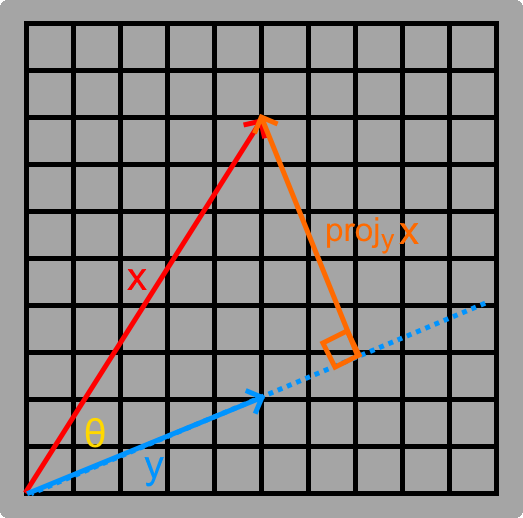
\includegraphics[scale=0.4]{Images/1.1.7.png}
    \end{figure}

    \vspace{0.5cm}



    \begin{example}
        Let x = (-4,5,7) and y = (2,-4,1). Find the vector decomposition
        of x onto y.
    \end{example}

    \begin{tbox}
        Parallel component:
        \hspace{0.5cm}
        $\text{proj}_yx$
        = $\frac{(-4*2 + 5*-4 + 7*1)}{2^2 + (-4)^2 + 1^2}(2,-4,1)$
        = $\frac{-21}{21}(2,-4,1)$ = (-2,4,-1)

        Orthogonal component:
        \hspace{0.5cm}
        x - $\text{proj}_yx$
        = (-4,5,7) - (-2,4,-1)
        = (-2,1,8)
    \end{tbox}

    \vspace{0.5cm}



    \begin{wtheorem}{Cauchy-Schwarz Inequality}{14cm}
        For x,y $\in$ $\mathbb{R}^n$,
        $|x \cdot y|$ $\leq$ $||x|| \ ||y||$
    \end{wtheorem}

    \begin{proof}
        Let y = proj$_xy$ + $x^{\perp}$ = cx + $x^{\perp}$
        where $x^{\perp}$ is the orthogonal component of y to x and
        proj$_xy$ = cx is the parallel component to x for some c $\in$ $\mathbb{R}$.

        \hspace{0.5cm}
        $x \cdot y$
        = $x \cdot (cx + x^{\perp})$
        = $c(x \cdot x) + x \cdot x^{\perp}$
        = $c||x||^2 + 0$
        = $c||x||^2$

        Thus, c = $\frac{x \cdot y}{||x||^2}$. Then:

        \hspace{0.5cm}
        $||y||^2$
        = $||cx+x^{\perp}||^2$
        = $(cx+x^{\perp}) \cdot (cx+x^{\perp})$
        = $cx \cdot cx + x^{\perp} \cdot x^{\perp} + 2(cx \cdot x^{\perp})$

        \hspace{1.5cm}
        = $c^2||x||^2 + ||x^{\perp}||^2$
        = $(\frac{x \cdot y}{||x||^2})^2 ||x||^2 + ||x^{\perp}||^2$

        \hspace{0.5cm}
        $||x||^2 ||y||^2$
        = $||x||^2(\frac{x \cdot y}{||x||^2})^2 ||x||^2 + ||x||^2 ||x^{\perp}||^2$
        = $(x \cdot y)^2 + ||x||^2 ||x^{\perp}||^2$

        Since $||x||^2 ||x^{\perp}||^2$ $\geq$ 0, then
        $(x \cdot y)^2$ $\leq$ $||x||^2 ||y||^2$
        so $|x \cdot y|$ $\leq$ $||x|| \ ||y||$.
    \end{proof}

    \vspace{0.5cm}



    \begin{wtheorem}{Triangle Inequality}{14cm}
        For x,y $\in$ $\mathbb{R}^n$,
        $||x+y||$ $\leq$ $||x|| + ||y||$
    \end{wtheorem}

    \begin{proof}
        $||x+y||^2$
        = $(x+y) \cdot (x+y)$
        = $x \cdot x + y \cdot y + 2(x \cdot y)$
        = $||x||^2 + ||y||^2 +2(x \cdot y)$

        \hspace{1.55cm}
        $\leq$ $||x||^2 + ||y||^2 +2|x \cdot y|$
        $\leq$ $||x||^2 + ||y||^2 +2||x|| \ ||y||$
        = $(||x|| + ||y||)^2$
    \end{proof}

    \newpage




\subsection{ Cross Product }

    \begin{definition}{Cross Product}{14cm}
        The {\color{lblue} cross product} of x,y $\in$ $\mathbb{R}^3$
        is the determinant of the standard basis, x, y:

        \hspace{0.5cm}
        $x \times y$ =
        det($
        \begin{bmatrix}
            e_1 & e_2 & e_3 \\
            x_1 & x_2 & x_3 \\
            y_1 & y_2 & y_3 
        \end{bmatrix}$)
        =
        $\begin{vmatrix}
            x_2 & x_3 \\
            y_2 & y_3 
        \end{vmatrix}e_1
        - \begin{vmatrix}
            x_1 & x_3 \\
            y_1 & y_3 
        \end{vmatrix}e_2
        + \begin{vmatrix}
            x_1 & x_2 \\
            y_1 & y_2 
        \end{vmatrix}e_3$
    \end{definition}

    \vspace{0.5cm}



    \begin{ltheorem}{Properties of the Cross Product}{1.5cm}
        \item $x \times y$ = $-(y \times x)$
        
            \begin{proof}[14cm]
                $x \times y$ =
                $\begin{vmatrix}
                    x_2 & x_3 \\
                    y_2 & y_3 
                \end{vmatrix}e_1
                - \begin{vmatrix}
                    x_1 & x_3 \\
                    y_1 & y_3 
                \end{vmatrix}e_2
                + \begin{vmatrix}
                    x_1 & x_2 \\
                    y_1 & y_2 
                \end{vmatrix}e_3$

                \hspace{1cm}
                = $-\begin{vmatrix}
                    y_2 & y_3 \\
                    x_2 & x_3 
                \end{vmatrix}e_1
                + \begin{vmatrix}
                    y_1 & y_3 \\
                    x_1 & x_3 
                \end{vmatrix}e_2
                - \begin{vmatrix}
                    y_1 & y_2 \\
                    x_1 & x_2 
                \end{vmatrix}e_3$
                = $-(y \times x)$
            \end{proof}
        
        \item $x \times (y + z)$ = $x \times y + x \times z$
        
            \begin{proof}[14cm]
                $x \times (y + z)$ =
                $\begin{vmatrix}
                    x_2 & x_3 \\
                    y_2+z_2 & y_3+z_3 
                \end{vmatrix}e_1
                - \begin{vmatrix}
                    x_1 & x_3 \\
                    y_1+z_1 & y_3+z_3 
                \end{vmatrix}e_2
                + \begin{vmatrix}
                    x_1 & x_2 \\
                    y_1+z_1 & y_2+z_2 
                \end{vmatrix}e_3$
                
                \hspace{0.1cm}
                = $(\begin{vmatrix}
                    x_2 & x_3 \\
                    y_2 & y_3 
                \end{vmatrix} +
                \begin{vmatrix}
                    x_2 & x_3 \\
                    z_2 & z_3 
                \end{vmatrix})e_1
                - (\begin{vmatrix}
                    x_1 & x_3 \\
                    y_1 & y_3 
                \end{vmatrix} +
                \begin{vmatrix}
                    x_1 & x_3 \\
                    z_1 & z_3 
                \end{vmatrix})e_2
                + (\begin{vmatrix}
                    x_1 & x_2 \\
                    y_1 & y_2 
                \end{vmatrix} +
                \begin{vmatrix}
                    x_1 & x_2 \\
                    z_1 & z_2 
                \end{vmatrix})e_3$

                \hspace{0.1cm}
                = $\begin{vmatrix}
                    x_2 & x_3 \\
                    y_2 & y_3 
                \end{vmatrix}e_1
                - \begin{vmatrix}
                    x_1 & x_3 \\
                    y_1 & y_3 
                \end{vmatrix}e_2
                + \begin{vmatrix}
                    x_1 & x_2 \\
                    y_1 & y_2 
                \end{vmatrix}e_3$
                + $\begin{vmatrix}
                    x_2 & x_3 \\
                    z_2 & z_3 
                \end{vmatrix}e_1
                - \begin{vmatrix}
                    x_1 & x_3 \\
                    z_1 & z_3 
                \end{vmatrix}e_2
                + \begin{vmatrix}
                    x_1 & x_2 \\
                    z_1 & z_2 
                \end{vmatrix}e_3$

                \hspace{0.1cm}
                = $x \times y + x \times z$
            \end{proof}

        \item $(x + y) \times z$ = $x \times z + y \times z$
        
            \begin{proof}[14cm]
                $(x + y) \times z$
                = $-[z \times (x+y)]$
                = $-[z \times x + z \times y]$

                \hspace{2cm}
                = $-[-(x \times z) + -(y \times z)]$
                = $x \times z + y \times z$
            \end{proof}

        \item $c(x \times y)$ = $cx \times y$ = $x \times cy$
        
            \begin{proof}[14cm]
                $c(x \times y)$ =
                $c\begin{vmatrix}
                    x_2 & x_3 \\
                    y_2 & y_3 
                \end{vmatrix}e_1
                - c\begin{vmatrix}
                    x_1 & x_3 \\
                    y_1 & y_3 
                \end{vmatrix}e_2
                + c\begin{vmatrix}
                    x_1 & x_2 \\
                    y_1 & y_2 
                \end{vmatrix}e_3$

                \hspace{1.5cm}
                = $\begin{vmatrix}
                    cx_2 & cx_3 \\
                    y_2 & y_3 
                \end{vmatrix}e_1
                - \begin{vmatrix}
                    cx_1 & cx_3 \\
                    y_1 & y_3 
                \end{vmatrix}e_2
                + \begin{vmatrix}
                    cx_1 & cx_2 \\
                    y_1 & y_2 
                \end{vmatrix}e_3$
                = $cx \times y$

                \hspace{1.5cm}
                = $\begin{vmatrix}
                    x_2 & x_3 \\
                    cy_2 & cy_3 
                \end{vmatrix}e_1
                - \begin{vmatrix}
                    x_1 & x_3 \\
                    cy_1 & cy_3 
                \end{vmatrix}e_2
                + \begin{vmatrix}
                    x_1 & x_2 \\
                    cy_1 & cy_2 
                \end{vmatrix}e_3$
                = $x \times cy$
            \end{proof}

        \item x $\times$ x = 0
        
            \begin{proof}[14cm]
                By part (a),
                x $\times$ x = -(x $\times$ x)
                \hspace{0.5cm}
                $\Rightarrow$
                \hspace{0.5cm}
                2(x $\times$ x) = 0
                \hspace{0.5cm}
                $\Rightarrow$
                \hspace{0.5cm}
                x $\times$ x = 0
            \end{proof}
    \end{ltheorem}

    \newpage



    \begin{wtheorem}{Orthgonality of $x \times y$}{14cm}
        $x \times y$ is orthogonal to x and y
    \end{wtheorem}

    \begin{proof}
        $x \times y$ $\cdot$ x =
        ($\begin{vmatrix}
            x_2 & x_3 \\
            y_2 & y_3 
        \end{vmatrix},
        - \begin{vmatrix}
            x_1 & x_3 \\
            y_1 & y_3 
        \end{vmatrix},
        \begin{vmatrix}
            x_1 & x_2 \\
            y_1 & y_2 
        \end{vmatrix}$)
        $\cdot$ $(x_1,x_2,x_3)$

        \hspace{1.6cm}
        = $(x_2y_3 - x_3y_2)x_1 - (x_1y_3 - x_3y_1)x_2 + (x_1y_2 - x_2y_1)x_3$

        \hspace{1.6cm}
        = $x_1x_2y_3 - x_1x_3y_2 - x_1x_2y_3 + x_2x_3y_1 + x_1x_3y_2 - x_2x_3y_1$
        = 0

        $x \times y$ $\cdot$ y =
        ($\begin{vmatrix}
            x_2 & x_3 \\
            y_2 & y_3 
        \end{vmatrix},
        - \begin{vmatrix}
            x_1 & x_3 \\
            y_1 & y_3 
        \end{vmatrix},
        \begin{vmatrix}
            x_1 & x_2 \\
            y_1 & y_2 
        \end{vmatrix}$)
        $\cdot$ $(y_1,y_2,y_3)$

        \hspace{1.6cm}
        = $(x_2y_3 - x_3y_2)y_1 - (x_1y_3 - x_3y_1)y_2 + (x_1y_2 - x_2y_1)y_3$

        \hspace{1.6cm}
        = $x_2y_1y_3 - x_3y_1y_2 - x_1y_2y_3 + x_3y_1y_2 + x_1y_2y_3 - x_2y_1y_3$
        = 0
    \end{proof}

    \vspace{0.5cm}



    \begin{example}
        Let x = (1,0,-3) and y = (6,8,2). Find an orthogonal vector to x and y.
    \end{example}

    \begin{tbox}
        $x \times y$
        = $\begin{vmatrix}
            e_1 & e_2 & e_3 \\
            1 & 0 & -3 \\
            6 & 8 & 2 
        \end{vmatrix}$
        = $((0*2 - 8*-3),(1*2 - 6*-3),(1*8 - 6*-0))$
        = (24,-20,8)
    \end{tbox}

    \vspace{0.5cm}



    \begin{wtheorem}{$||x \times y||$ = $||x|| \ ||y|| \sin(\theta)$}{14cm}
        For x,y $\in$ $\mathbb{R}^3$:
        
        \hspace{0.5cm}
        $||x \times y||$ = $||x|| \ ||y|| \sin(\theta)$

        where $\theta$ $\in$ $[0,\pi]$ is the angle between x and y
    \end{wtheorem}

    \begin{proof}
        By {\color{red} theorem 1.2.3},
        $x \cdot y$ = $||x|| \ ||y|| \cos(\theta)$
        where $\theta$ $\in$ $[0,\pi]$ is the angle between x,y.

        \hspace{0.5cm}
        $||x||^2 ||y||^2 - (x \cdot y)^2$
        = $||x||^2 ||y||^2 (1 - \cos^2(\theta))$
        = $||x||^2 ||y||^2 \sin^2(\theta)$

        Also:

        \hspace{0.5cm}
        $||x||^2 ||y||^2 - (x \cdot y)^2$
        = $(x_1^2 + x_2^2 + x_3^2)(y_1^2 + y_2^2 + y_3^2)
            - (x_1y_1 + x_2y_2 + x_3y_3)^2$

        \hspace{0.5cm}
        = $(x_1^2y_1^2 + x_2^2y_2^2 + x_3^2y_3^2
            + {\color{green} x_1^2y_2^2} + {\color{lblue} x_1^2y_3^2}
            + {\color{green} x_2^2y_1^2} + {\color{red} x_2^2y_3^2}
            + {\color{lblue} x_3^2y_1^2} + {\color{red} x_3^2y_2^2}$

            \hspace{1cm}
            $- x_1^2y_1^2 - x_2^2y_2^2 - x_3^2y_3^2
            - {\color{green} 2x_1x_2y_1y_2}
            - {\color{lblue} 2x_1x_3y_1y_3}
            - {\color{red} 2x_2x_3y_2y_3})$

        \hspace{0.5cm}
        = ${\color{red} (x_2y_3 - x_3y_2)^2}
            + {\color{lblue} (x_3y_1 - x_1y_3)^2}
            + {\color{green} (x_1y_2 - x_2y_1)^2}$
        = $||x \times y||^2$

        Thus, $||x \times y||$ = $||x|| \ ||y|| \sin(\theta)$.
    \end{proof}

    \newpage



    \begin{wtheorem}{Area of Parallelogram}{14cm}
        The area of a parallelogram P with sides x,y $\in$ $\mathbb{R}^3$:

        \hspace{0.5cm}
        $\text{Vol}_2(P(x,y))$ = $||x \times y||$
    \end{wtheorem}

    \begin{proof}
        Since parallelogram P with sides x and y is two triangles with
        sides x and y, then:

        \hspace{0.5cm}
        $\text{Vol}_2(P(x,y))$
        = 2 * $\text{Vol}_2(\text{Triangle}(x,y))$
        
        \hspace{3cm}
        = 2 * $\frac{1}{2}$ (base of triangle) * (height of triangle)
      
        \hspace{3cm}
        = $||x|| * (||y||\sin(\theta))$
        = $||x \times y ||$
    \end{proof}

    \begin{figure}[h]
        \centering
        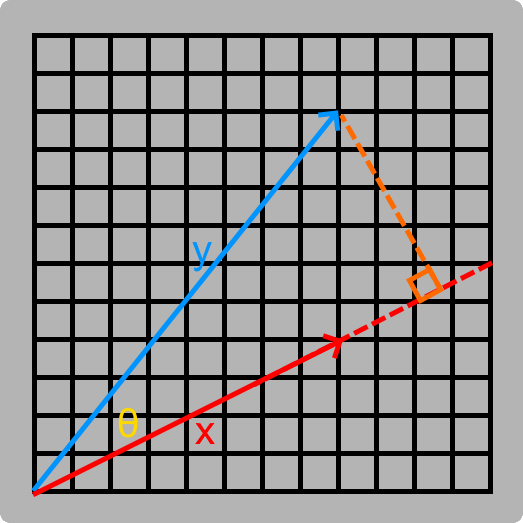
\includegraphics[scale=0.4]{Images/1.3.5.png}        
    \end{figure}



    \begin{wtheorem}{Volume of Parallelepiped}{14cm}
        The volume of a parallelepiped P with sides x,y,z $\in$ $\mathbb{R}^n$:

        \hspace{0.5cm}
        Vol$_3(P(x,y,z))$
        = $|(x \times y) \cdot z|$
    \end{wtheorem}

    \begin{proof}
        Let sides x and y form a base for P.

        \hspace{0.5cm}
        Vol$_3(P(x,y,z))$
        = (Area of base) * (height)
        = $||x \times y|| * (||z|| \cos(\theta))$

        where $\theta$ $\in$ $[0,\pi]$ is the angle between $x \times y$
        and z. By {\color{red} theorem 1.2.3}:

        \hspace{0.5cm}
        Vol$_3(P(x,y,z))$ = $(x \times y) \cdot z$

        Since -1 $\leq$ cos($\theta$) $\leq$ 1 for $\theta$ $\in$ $[0,2\pi]$, then
        $(x \times y) \cdot z$ can be negative. Thus:

        \hspace{0.5cm}
        Vol$_3(P(x,y,z))$ = $|(x \times y) \cdot z|$
    \end{proof}

    \begin{figure}[h]
        \centering
        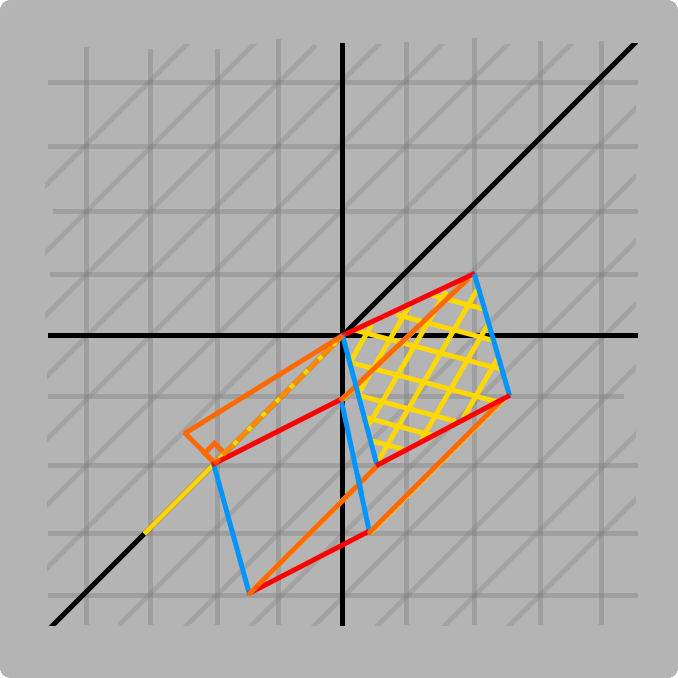
\includegraphics[scale=0.3]{Images/1.3.6.png}
    \end{figure}

    \newpage





\subsection{ Distances and Planes }

    \begin{wtheorem}{Equation of a Plane: Method \#1: Point and Normal Vector}{14cm}
        A plane in $\mathbb{R}^3$ through a point p = $(p_x,p_y,y_z)$
        and orthogonal to a vector called a normal vector
        n = $(a,b,c)$ has an equation of the form:

        \hspace{0.5cm}
        n $\times$ $[(x,y,z)-p]$ = $a(x-p_x) + b(y-p_y) + c(z-p_z)$ = 0
    \end{wtheorem}

    \begin{proof}
        Let (x,y,z) be any point in the plane.
        Then (x,y,z) - p = $(x-p_x,y-p_y,z-p_z)$ is a vector
        parallel to the plane. Since the plane is orthogonal to vector n,
        then any vector parallel to the plane is orthogonal to n. Thus:

        \hspace{0.5cm}
        $n \cdot (x-p_x,y-p_y,z-p_z)$ = 0

        \hspace{0.5cm}
        $ a(x-p_x) + b(y-p_y) + c(z-p_z)$ = 0
    \end{proof}

    \begin{figure}[h]
        \centering
        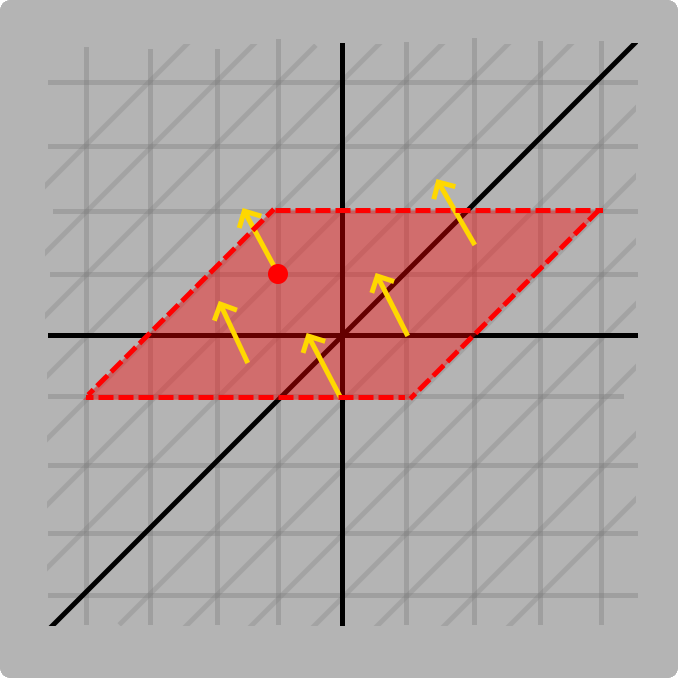
\includegraphics[scale=0.3]{Images/1.4.1.png}
    \end{figure}



    \begin{wtheorem}{Equation of a Plane: Method \#2: 3 Points}{14cm}
        A plane in $\mathbb{R}^3$ through points
        $p_1 = (x_1,y_1,z_1)$, $p_2 = (x_2,y_2,z_2)$, and $p_3 = (x_3,y_3,z_3)$
        has an equation of the form:

        \hspace{0.5cm}
        $[(p_2 - p_1) \times (p_3 - p_1)] \cdot [(x,y,z) - p_1]$ = 0
    \end{wtheorem}

    \begin{proof}
        Since $p_1$, $p_2$, and $p_3$ are on the plane, then
        $p_2-p_1$ and $p_3-p_1$ are vectors on the plane and thus, parallel to
        the plane.
        Since $(p_2 - p_1) \times (p_3 - p_1)$ is orthgonal to
        $(p_2 - p_1)$ and $(p_3 - p_1)$, then $(p_2 - p_1) \times (p_3 - p_1)$
        is orthogonal to the plane and thus, a normal vector.
        By {\color{red} theorem 1.4.1}, then
        $[(p_2 - p_1) \times (p_3 - p_1)] \cdot [(x,y,z) - p_1]$ = 0.
    \end{proof}

    \begin{figure}[h]
        \centering
        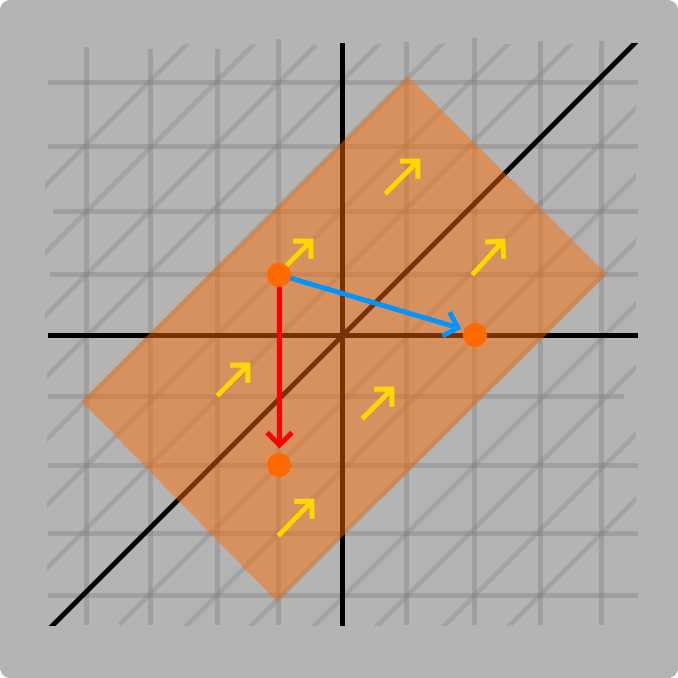
\includegraphics[scale=0.3]{Images/1.4.2.png}
    \end{figure}

    \newpage



    \begin{wtheorem}{Distance: Point + Line or 2 Parallel Lines}{14cm}
        The distance from line L(t) = tv+$x_0$ to point p $\in$ $\mathbb{R}^3$
        where t $\in$ $\mathbb{R}$, v,$x_0$ $\in$ $\mathbb{R}^3$:

        \hspace{0.5cm}
        $\frac{||v \times (p - x_0)||}{||v||}$

        If line $L_2(t)$ is parallel to L(t), choose a point on $L_2(t)$
        and apply formula above to get the distance between two parallel lines.
    \end{wtheorem}

    \begin{proof}
        Since $x_0$ is a point on L(t), then
        $p - x_0$ is a vector from line L(t) to p.

        Let $\theta$ be the angle between $p - x_0$
        and L(t). Thus:

        \hspace{0.5cm}
        sin($\theta$) = $\frac{d}{||p - x_0||}$
        \hspace{0.5cm}
        $\Rightarrow$
        \hspace{0.5cm}
        d = $||p - x_0|| * \sin(\theta)$
        = $\frac{||v|| * ||p - x_0|| * \sin(\theta)}{||v||}$
        = $\frac{||v \times (p - x_0)||}{||v||}$
    \end{proof}

    \begin{figure}[h]
        \centering
        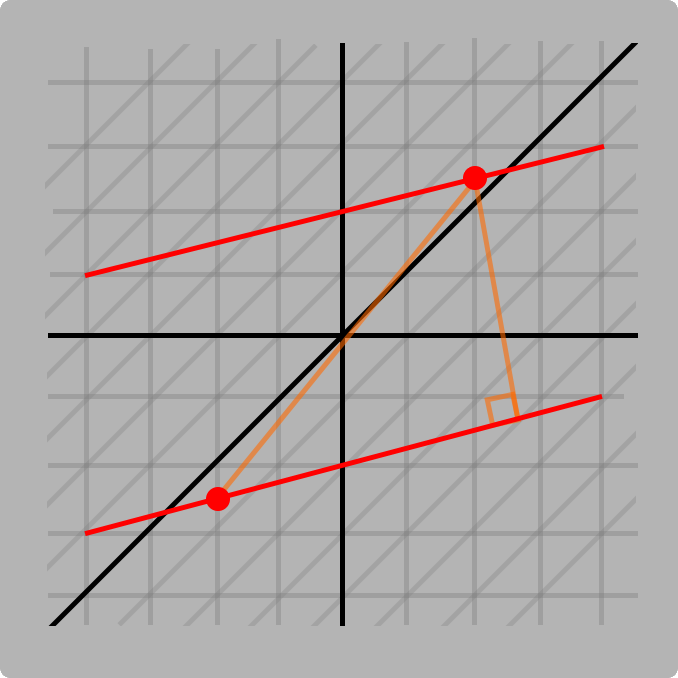
\includegraphics[scale=0.3]{Images/1.4.3.png}
    \end{figure}



    \begin{wtheorem}{Distance: Parallel Planes}{14cm}
        The distance between parallel planes
        $P_1$: $a(x-x_1) + b(y-y_1) + c(z-z_1)$ = 0
        and $P_2$: $a(x-x_2) + b(y-y_2) + c(z-z_2)$ = 0:

        \hspace{0.5cm}
        d = $\frac{|(a,b,c) \cdot (x_2-x_1,y_2-y_1,z_2-z_1)|}{\sqrt{a^2+b^2+c^2}}$
    \end{wtheorem}

    \begin{proof}
        Planes $P_1$ and $P_2$ are parallel since they both have the normal vector
        n = (a,b,c).
        Since $(x_1,y_1,z_1)$ is a point on $P_1$ and
        $(x_2,y_2,z_2)$ is a point on $P_2$, then
        $(x_2,y_2,z_2) - (x_1,y_1,z_1)$ is a vector from $P_1$ to $P_2$.

        Then the distance is the norm of the orthogonal component of
        $(x_2,y_2,z_2) - (x_1,y_1,z_1)$ to $P_1,P_2$.
        Since normal vector n is orthogonal to both planes, then
        the orthogonal component of $(x_2,y_2,z_2) - (x_1,y_1,z_1)$
        and n are parallel.
        Thus, by {\color{red} theorem 1.2.4}:

        \hspace{0.5cm}
        d = $||\text{proj}_n[(x_2,y_2,z_2) - (x_1,y_1,z_1)]|$
        = $||\frac{[(x_2,y_2,z_2) - (x_1,y_1,z_1)] \cdot (a,b,c)}
                    {||(a,b,c)||^2}(a,b,c)||$

        \hspace{0.5cm}
        d = $\frac{|(x_2-x_1,y_2-y_1,z_2-z_1) \cdot (a,b,c)|}
        {||(a,b,c)||}$
    \end{proof}

    \begin{figure}[h]
        \centering
        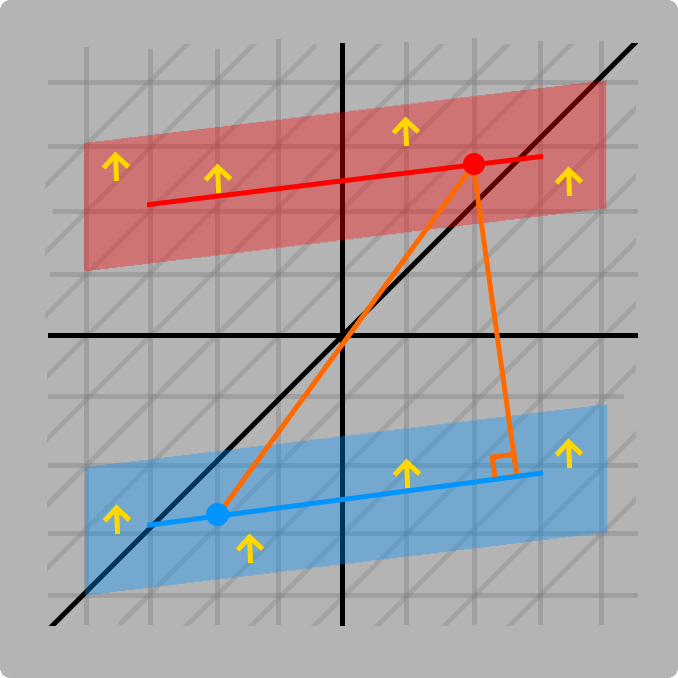
\includegraphics[scale=0.3]{Images/1.4.4.png}
    \end{figure}

    \newpage



    \begin{wtheorem}{Distance: Skew Lines}{14cm}
        Lines $L_1,L_2 \in \mathbb{R}^3$ are skewed if they are neither parallel
        or intersecting.

        Let $L_1(t)$ = $tv_1 + x_1$ and $L_1(t)$ = $tv_2 + x_2$.
        The distance between $L_1$ and $L_2$:

        \hspace{0.5cm}
        d = $\frac{| (v_2 \times v_1) \cdot (x_2-x_1) |}{||v_2 \times v_1||}$
    \end{wtheorem}

    \begin{proof}
        Let $L_1,L_2$ be in two parallel planes.
        Note the distance between $L_1$ and $L_2$ is the distance between
        the two planes.

        Since $v_2 \times v_1$ is orthogonal to $v_1,v_2$ and $v_1,v_2$ are
        vectors parallel to each plane, then $v_2 \times v_1$ is orthogonal to
        each plane and thus, a normal vector.
        By {\color{red} theorem 1.4.4}:

        \hspace{0.5cm}
        d = $\frac{| (v_2 \times v_1) \cdot (x_2-x_1) |}{||v_2 \times v_1||}$
    \end{proof}

    \begin{figure}[h]
        \centering
        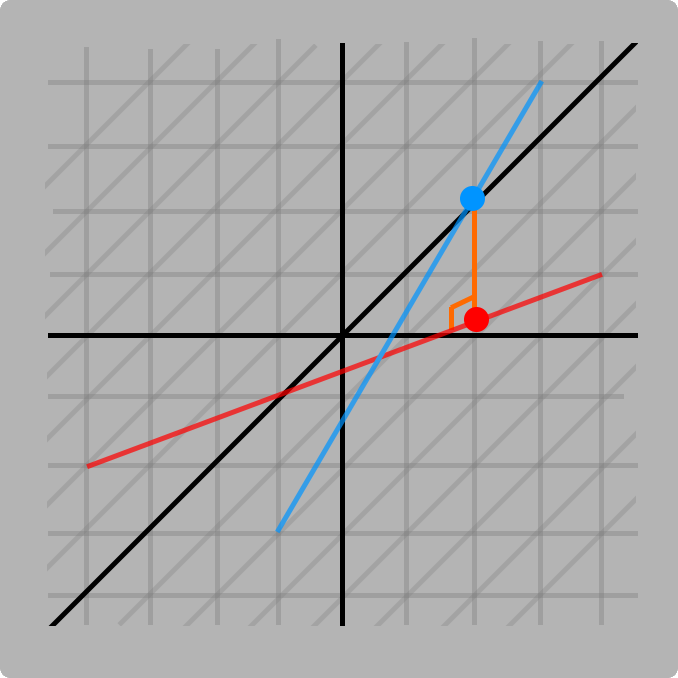
\includegraphics[scale=0.3]{Images/1.4.5.png}
    \end{figure}





\subsection{ Matrices }

    \begin{definition}{Matrix}{14cm}
        A {\color{lblue} m by n matrix} $M_{m \times n}(\mathbb{R})$:

        \hspace{0.5cm}
        M =
        $\begin{bmatrix}
            a_{11} & a_{12} & \hdots & a_{1n} \\
            
            a_{21} & a_{22} & \hdots & a_{2n} \\
            
            \vdots & \vdots & \ddots & \vdots \\
            
            a_{m1} & a_{m2} & \hdots & a_{mn} \\
        \end{bmatrix}$
        \hspace{1cm}
        where each $a_{ij}$ $\in$ $\mathbb{R}$

        \vspace{0.3cm}



        A {\color{lblue} row vector} is a 1 by n matrix:

        \hspace{0.5cm}
        $\begin{bmatrix}
            a_{11}
            & a_{12}
            & \hdots
            & a_{1n}
        \end{bmatrix}$

        \vspace{0.3cm}



        A {\color{lblue} column vector} is a m by 1 matrix:

        \hspace{0.5cm}
        $\begin{bmatrix}
            a_{11} \\
            a_{21} \\
            \vdots \\
            a_{m1} \\
        \end{bmatrix}$

        \vspace{0.3cm}



        A {\color{lblue} zero matrix} 0 $\in$ $M_{m \times n}(\mathbb{R})$:

        \hspace{0.5cm}
        0 = 
        $\begin{bmatrix}
            0_{11} & 0_{12} & \hdots & 0_{1n} \\

            0_{21} & 0_{22} & \hdots & 0_{2n} \\

            \vdots & \vdots & \ddots & \vdots \\
            
            0_{m1} & 0_{m2} & \hdots & 0_{mn} \\
        \end{bmatrix}$
    \end{definition}

    \newpage



    \begin{ltheorem}{Matrix Operations}{1.5cm}
        \item Addition

            For A,B $\in$ $M_{m \times n}(\mathbb{R})$,
            then A+B $\in$ $M_{m \times n}(\mathbb{R})$
            where each $a_{ij},b_{ij}$:
        
            {\footnotesize
            $
            \begin{bmatrix}
                a_{11} & a_{12} & \hdots & a_{1n} \\
                a_{21} & a_{22} & \hdots & a_{2n} \\
                \vdots & \vdots & \ddots & \vdots \\
                a_{m1} & a_{m2} & \hdots & a_{mn} \\
            \end{bmatrix} +
            \begin{bmatrix}
                b_{11} & b_{12} & \hdots & b_{1n} \\
                b_{21} & b_{22} & \hdots & b_{2n} \\
                \vdots & \vdots & \ddots & \vdots \\
                b_{m1} & b_{m2} & \hdots & b_{mn} \\
            \end{bmatrix}
            $
            =
            $
            \begin{bmatrix}
                a_{11}+b_{11} & a_{12}+b_{12} & \hdots & a_{1n}+b_{1n} \\
                a_{21}+b_{21} & a_{22}+b_{22} & \hdots & a_{2n}+b_{2n} \\
                \vdots & \vdots & \ddots & \vdots \\
                a_{m1}+b_{m1} & a_{m2}+b_{m2} & \hdots & a_{mn}+b_{mn} \\
            \end{bmatrix}
            $}

        \item Scalar Multiplication
            
            For A $\in$ $M_{m \times n}(\mathbb{R})$,
            then cA $\in$ $\in$ $M_{m \times n}(\mathbb{R})$
            where each $a_{ij},b_{ij}$:

            {\footnotesize
            $c
            \begin{bmatrix}
                a_{11} & a_{12} & \hdots & a_{1n} \\
                a_{21} & a_{22} & \hdots & a_{2n} \\
                \vdots & \vdots & \ddots & \vdots \\
                a_{m1} & a_{m2} & \hdots & a_{mn} \\
            \end{bmatrix}$
            =
            $
            \begin{bmatrix}
                ca_{11} & ca_{12} & \hdots & ca_{1n} \\
                ca_{21} & ca_{22} & \hdots & ca_{2n} \\
                \vdots & \vdots & \ddots & \vdots \\
                ca_{m1} & ca_{m2} & \hdots & ca_{mn} \\
            \end{bmatrix}
            $}
        
        \item Multiplication
        
            For A $\in$ $M_{m \times n}(\mathbb{R})$,
            B $\in$ $M_{n \times k}(\mathbb{R})$,
            then AB $\in$ $M_{m \times k}(\mathbb{R})$
            where each $a_{ij},b_{ij}$:
            
            {\footnotesize
            $
            \begin{bmatrix}
                {\color{red} a_{11}} & {\color{red} a_{12}}
                                    & \hdots & {\color{red} a_{1n}} \\
                {\color{lblue} a_{21}} & {\color{lblue} a_{22}}
                                    & \hdots & {\color{lblue} a_{2n}} \\
                \vdots & \vdots & \ddots & \vdots \\
                {\color{green} a_{m1}} & {\color{green} a_{m2}}
                                    & \hdots & {\color{green} a_{mn}} \\
            \end{bmatrix}
            \begin{bmatrix}
                {\color{orange} b_{11}} & {\color{magenta} b_{12}}
                                        & \hdots & {\color{pink} b_{1k}} \\
                {\color{orange} b_{21}} & {\color{magenta} b_{22}} 
                                        & \hdots & {\color{pink} b_{2k}} \\
                \vdots & \vdots & \ddots & \vdots \\
                {\color{orange} b_{n1}} & {\color{magenta} b_{n2}}
                                        & \hdots & {\color{pink} b_{nk}} \\
            \end{bmatrix}
            $}
            =
            {\footnotesize
            $
            \begin{bmatrix}
                \sum_{i=1}^n {\color{red} a_{1i}} {\color{orange} b_{i1}}
                & \sum_{i=1}^n {\color{red} a_{1i}} {\color{magenta} b_{i2}}
                & \hdots
                & \sum_{i=1}^n {\color{red} a_{1i}} {\color{pink} b_{ik}} \\

                \sum_{i=1}^n {\color{lblue} a_{2i}} {\color{orange} b_{i1}}
                & \sum_{i=1}^n {\color{lblue} a_{2i}} {\color{magenta} b_{i2}}
                & \hdots
                & \sum_{i=1}^n {\color{lblue} a_{2i}} {\color{pink} b_{ik}} \\
                
                \vdots & \vdots & \ddots & \vdots \\

                \sum_{i=1}^n {\color{green} a_{mi}} {\color{orange} b_{i1}}
                & \sum_{i=1}^n {\color{green} a_{mi}} {\color{magenta} b_{i2}}
                & \hdots
                & \sum_{i=1}^n {\color{green} a_{mi}} {\color{pink} b_{ik}} \\
            \end{bmatrix}$}
    \end{ltheorem}

    \vspace{0.5cm}



    \begin{ltheorem}{Properties of Matrix Operations}{1.5cm}
        \item A+B = B+A
        
            \begin{proof}[14cm]
                $[A+B]_{ij}$ = $a_{ij} + b_{ij}$
                = $b_{ij} + a_{ij}$ = $[B+A]_{ij}$
            \end{proof}
        
        \item A+(B+C) = (A+B)+C
        
            \begin{proof}[14cm]
                $[A+(B+C)]_{ij}$ = $a_{ij} + (b_{ij} + c_{ij})$
                = $(a_{ij} + b_{ij}) + c_{ij}$ = $[(A+B)+C]_{ij}$
            \end{proof}
        
        \item A+0 = A
        
            \begin{proof}[14cm]
                $[A+0]_{ij}$ = $a_{ij} + 0_{ij}$
                = $a_{ij}$ = $[A]_{ij}$
            \end{proof}
        
        \item (c+k)A = cA + kA
            
            \begin{proof}[14cm]
                $[(c+k)A]_{ij}$ = $(c+k)a_{ij}$
                = $ca_{ij} + ka_{ij}$ = $[cA]_{ij} + [kA]_{ij}$
                = $[cA + kA]_{ij}$
            \end{proof}
        
        \item c(A+B) = cA + cB
        
            \begin{proof}[14cm]
                $[c(A+B)]_{ij}$ = $c(a_{ij} + b_{ij})$
                = $ca_{ij} + cb_{ij}$ = $[cA]_{ij} + [cB]_{ij}$
                = $[cA+cB]_{ij}$
            \end{proof}

        \item c(kA) = (ck)A = k(cA)
        
            \begin{proof}[14cm]
                $[c(kA)]_{ij}$
                = $c(ka_{ij})$
                = $(ck)a_{ij}$
                = $[(ck)A]_{ij}$
                = $k(ca_{ij})$
                = $[k(cA)]_{ij}$
            \end{proof}

            \newpage
        
        \item A(BC) = (AB)C
        
            \begin{proof}[14cm]
                Let A $\in$ $M_{m \times n}(\mathbb{R})$,
                B $\in$ $M_{n \times k}(\mathbb{R})$,
                and C $\in$ $M_{k \times p}(\mathbb{R})$.

                For u $\in$ \{1,...,n\} and v $\in$ \{1,...,p\}, then
                [BC]$_{uv}$ = $\sum_{s=1}^k b_{us}c_{sv}$.

                Thus, for i $\in$ \{1,...,m\} and j $\in$ \{1,...,p\}:

                \hspace{0.2cm}
                $[A(BC)]_{ij}$ = $\sum_{t=1}^n a_{it}[BC]_{tj}$
                = $\sum_{t=1}^n [a_{it} \sum_{s=1}^k b_{ts}c_{sj}]$
                = $\sum_{t=1}^n \sum_{s=1}^k a_{it}b_{ts}c_{sj}$

                \hspace{0.2cm}
                = $\sum_{s=1}^k \sum_{t=1}^n a_{it}b_{ts}c_{sj}$
                = $\sum_{s=1}^k [\sum_{t=1}^n a_{it}b_{ts}]c_{sj}$
                = $\sum_{s=1}^k [AB]_{is} c_{sj}$
                = $[(AB)C]_{ij}$
            \end{proof}
        
        \item c(AB) = (cA)B = A(cB)
        
            \begin{proof}[14cm]
                Let A $\in$ $M_{m \times n}(\mathbb{R})$ and
                B $\in$ $M_{n \times k}(\mathbb{R})$.
                For i $\in$ \{1,...,m\} and j $\in$ \{1,...,k\}:

                \hspace{0.5cm}
                $[c(AB)]_{ij}$ = $c\sum_{t=1}^n a_{it}b_{tj}$
                = $\sum_{t=1}^n ca_{it}b_{tj}$
                = $\sum_{t=1}^n (ca_{it})b_{tj}$
                = $[(cA)B]_{ij}$

                \hspace{0.5cm}
                $[c(AB)]_{ij}$ = $c\sum_{t=1}^n a_{it}b_{tj}$
                = $\sum_{t=1}^n a_{it}cb_{tj}$
                = $\sum_{t=1}^n a_{it}(cb_{tj})$
                = $[A(cB)]_{ij}$
            \end{proof}

        \item A(B+C) = AB + AC
        
            \begin{proof}[14cm]
                Let A $\in$ $M_{m \times n}(\mathbb{R})$ and
                B,C $\in$ $M_{n \times k}(\mathbb{R})$.
                For i $\in$ \{1,...,m\} and j $\in$ \{1,...,k\}:

                \hspace{0.5cm}
                $[A(B+C)]_{ij}$ = $\sum_{t=1}^n a_{it}[B+C]_{tj}$
                = $\sum_{t=1}^n a_{it}(b_{tj}+c_{tj})$
                = $\sum_{t=1}^n a_{it}b_{tj} + a_{it}c_{tj}$

                \hspace{0.5cm}
                = $\sum_{t=1}^n a_{it}b_{tj}$ + $\sum_{t=1}^n a_{it}c_{tj}$
                = $[AB]_{ij} + [AC]_{ij}$
                = $[AB + AC]_{ij}$
            \end{proof}
        
        \item (A+B)C = AC + BC
        
            \begin{proof}[14cm]
                Let A,B $\in$ $M_{m \times n}(\mathbb{R})$ and
                C $\in$ $M_{n \times k}(\mathbb{R})$.
                
                For i $\in$ \{1,...,m\} and j $\in$ \{1,...,k\},
                the ij-th entry for (A+B)C:

                \hspace{0.5cm}
                $[(A+B)C]_{ij}$ = $\sum_{t=1}^n [A+B]_{it}c_{tj}$
                = $\sum_{t=1}^n (a_{it}+b_{it})c_{tj}$
                = $\sum_{t=1}^n a_{it}c_{tj} + b_{it}c_{tj}$

                \hspace{0.5cm}
                = $\sum_{t=1}^n a_{it}c_{tj}$ + $\sum_{t=1}^n b_{it}c_{tj}$
                = $[AC]_{ij} + [BC]_{ij}$
                = $[AC + BC]_{ij}$
            \end{proof}
    \end{ltheorem}

    \vspace{0.5cm}



    \begin{definition}{Transpose}{14cm}
        For matrix A $\in$ $M_{m \times n}(\mathbb{R})$:
        
        \hspace{0.5cm}
        A =
        $
        \begin{bmatrix}
            {\color{red} a_{11}} & {\color{red} a_{12}}
                    & {\color{red} a_{13}} & \hdots & {\color{red} a_{1n}} \\
            {\color{lblue} a_{21}} & {\color{lblue} a_{22}}
                    & {\color{lblue} a_{23}} & \hdots & {\color{lblue} a_{2n}} \\
            {\color{green} a_{31}} & {\color{green} a_{32}} 
                    & {\color{green} a_{33}} & \hdots & {\color{green} a_{3n}} \\
            \vdots & \vdots & \vdots & \ddots & \vdots \\
            {\color{orange} a_{m1}} & {\color{orange} a_{m2}} 
                    & {\color{orange} a_{m3}} & \hdots & {\color{orange} a_{mn}} \\
        \end{bmatrix}
        $
        
        then the {\color{lblue} transpose},
        $A^T$ $\in$ $M_{n \times m}(\mathbb{R})$:

        \hspace{0.5cm}
        $A^T$ =
        $
        \begin{bmatrix}
            {\color{red} a_{11}} & {\color{lblue} a_{21}}
                    & {\color{green} a_{31}} & \hdots & {\color{orange} a_{m1}} \\
            {\color{red} a_{12}} & {\color{lblue} a_{22}}
                    & {\color{green} a_{32}} & \hdots & {\color{orange} a_{m2}} \\
            {\color{red} a_{13}} & {\color{lblue} a_{23}}
                    & {\color{green} a_{33}} & \hdots & {\color{orange} a_{m3}} \\
            \vdots & \vdots & \vdots & \ddots & \vdots \\
            {\color{red} a_{1n}} & {\color{lblue} a_{2n}}
                    & {\color{green} a_{3n}} & \hdots & {\color{orange} a_{mn}} \\
        \end{bmatrix}
        $
    \end{definition}

    \newpage



    \begin{ltheorem}{Properties of the Transpose}{1.5cm}
        \item $(A^T)^T$ = A
        
            \begin{proof}[14cm]
                $[(A^T)^T]_{ij}$
                = $[A^T]_{ji}$
                = $[A]_{ij}$
            \end{proof}
        
        \item $(AB)^T$ = $B^T A^T$
        
            \begin{proof}[14cm]
                Let A $\in$ $M_{m \times n}(\mathbb{R})$ and
                B $\in$ $M_{n \times k}(\mathbb{R})$.
                For i = \{1,...,k\} and j = \{1,...,m\}:

                \hspace{0.5cm}
                $[(AB)^T]_{ij}$
                = $[AB]_{ji}$
                = $\sum_{t=1}^n a_{jt}b_{ti}$
                = $\sum_{t=1}^n b_{ti}a_{jt}$
                = $\sum_{t=1}^n b^T_{it}a^T_{tj}$
                = $[B^T A^T]_{ij}$
            \end{proof}

        \item $x \cdot y$ = $x^T y$
        
            \begin{proof}[14cm]
                $x \cdot y$
                = $x_1y_1 + x_2y_2 + ... + x_ny_n$
                = $[x_1 \ x_2 \ ... \ x_n]y$
                = $x^Ty$
            \end{proof}
    \end{ltheorem}

    \vspace{0.5cm}



    \begin{definition}{Determinant}{14cm}
        For A $\in$ $M_{n \times n}(\mathbb{R})$,
        let prod(A) = $a_{1,j_1} * a_{2,j_2} * ... * a_{n,j_n}$
        such that for any two $a_{k,j_k}$,$a_{p,j_p}$ where k $<$ p,
        then $j_k$ $\not =$ $j_p$.
        Let prod(A) be unique in the sense that no two prod(A)
        have exactly the same \{$a_{1,j_1}, a_{2,j_2}, ... , a_{n,j_n}$\}.

        Also, for any two such $a_{k,j_k}$,$a_{p,j_p}$,
        let an inversion be 1 if $j_k < j_p$ and 0 if $j_k > j_p$.
        Then for any prod(A), associate a sign(A)
        = $(-1)^{\text{total number of inversions in prod(A)}}$.

        Then the {\color{lblue} determinant} of A:

        \hspace{0.5cm}
        det(A) = $\sum_{\text{all prod(A)}} \text{prod(A) * sign(A)}$
    \end{definition}

    \vspace{0.5cm}



    \begin{example}
        Let A =
        $
        \begin{bmatrix}
            1 & 2 & 3 \\
            -1 & 1 & 1 \\
            5 & -2 & 3 
        \end{bmatrix}
        $.
        Find the det(A).
    \end{example}

    \begin{tbox}
        det(A) =
        (1*1*3)$(-1)^0$
        + (1*-2*1)$(-1)^1$
        + (-1*2*3)$(-1)^1$
        + (-1*-2*3)$(-1)^2$

        \hspace{1.7cm}
        + (5*2*1)$(-1)^2$
        + (5*1*3)$(-1)^3$
        = 12
    \end{tbox}

    \newpage



    \begin{wtheorem}{Cofactor Expansion}{14cm}
        Let A $\in$ $M_{n \times n}(\mathbb{R})$.
        Let $A_{ij}$ be A, but the i-th row and j-th column removed.

        Then for a fixed i $\in$ \{1,...,n\}:

        \hspace{0.5cm}
        det(A) = $(-1)^{i+1}a_{i1}\text{det}(A_{i1})
                    + (-1)^{i+2}a_{i2}\text{det}(A_{i2})
                    + ... + (-1)^{i+n}a_{in}\text{det}(A_{in})$

        Or for a fixed j $\in$ \{1,...,n\}:

        \hspace{0.5cm}
        det(A) = $(-1)^{1+j}a_{1j}\text{det}(A_{1j})
                    + (-1)^{2+j}a_{2j}\text{det}(A_{2j})
                    + ... + (-1)^{n+j}a_{nj}\text{det}(A_{nj})$
    \end{wtheorem}

    \begin{proof}
        For any n by n matrix A, each prod(A) must contain n $a_{ij}$
        where each $a_{ij}$'s i,j is different from another $a_{ij}$'s i,j.
        Thus, each prod(A) must contain only one $a_{ij}$ in each row and column.
        
        There are n possibles $a_{ij}$ choices in the first column and by choosing
        any such one, then that row is eliminated for choice in the following
        columns. Thus, there are n-1 possible $a_{ij}$ choices in the second column
        and by choosing any such one, then that row is also eliminated for choice
        in the following columns. Repeating the pattern, then
        there are n*(n-1)*(n-2)*...*1 = n! total unique prod(A) combinations.
        In the cofactor expansion, let choose a fixed i. The case for a fixed j
        is analogous.
        For a fixed i, the cofactor expansion iterates through each of the n
        columns in row i so there are n unique $a_{ij}$.
        For each $a_{ij}$, the $A_{ij}$ has the i-th row and j-th column
        removed so $A_{ij}$ is a (n-1) by (n-1) matrix and thus, there
        are (n-1)! unique prod($A_{ij}$) combinations as proved earlier.
        Since each $A_{ij}$ removes a different j-th column, then each
        prod($A_{ij}$) from different columns are unique.
        Thus, the n unique $a_{ij}$ has (n-1)! unique prod($A_{ij}$) combinations
        so there are n*(n-1)! = n! unique prod(A) combinations.
        Thus, the prod(A) combinations in the cofactor expansion must be equivalent
        to the prod(A) combinations in the original determinant.

        For the fixed i, let fixed j $\in$ \{1,...,n\}:

        \hspace{0.5cm}
        $
        \begin{bmatrix}
            a_{1,1} & a_{1,2} & a_{1,3} & \hdots
                    & a_{1,j-1} & {\color{lblue} a_{1,j}}
                    & a_{1,j+1} & \hdots & a_{1,n} \\
            \vdots & \vdots & \vdots & \ddots
                    & \vdots & \vdots & \vdots & \ddots & \vdots \\
            a_{i-1,1} & a_{i-1,2} & a_{i-1,3} & \hdots
                    & a_{i-1,j-1} & {\color{lblue} a_{i-1,j}}
                    & a_{i-1,j+1} & \hdots & a_{i-1,n} \\
            {\color{red} a_{i,1}} & {\color{red} a_{i,2}} & {\color{red} a_{i,3}}
                & \hdots & {\color{red} a_{i,j-1}} & {\color{purple} a_{i,j}}
                & {\color{red} a_{i,j+1}} & \hdots & {\color{red} a_{i,n}} \\
            a_{i+1,1} & a_{i+1,2} & a_{i+1,3} & \hdots
                    & a_{i+1,j-1} & {\color{lblue} a_{i+1,j}}
                    & a_{i+1,j+1} & \hdots & a_{i+1,n} \\
            \vdots & \vdots & \vdots & \ddots
                    & \vdots & \vdots & \vdots & \ddots & \vdots \\
            a_{n,1} & a_{n,2} & a_{n,3} & \hdots
                    & a_{n,j-1} & {\color{lblue} a_{n,j}}
                    & a_{n,j+1} & \hdots & a_{n,n} \\
        \end{bmatrix}
        $

        In the original determinant, each prod(A) associates
        sign(A) = $(-1)^{\text{\tiny \# inversions in prod(A)}}$.
        As proven earlier, each prod(A) is expressed in the coefactor expansion.
        So for any prod(A) that contains $a_{ij}$ with the fixed i,j, then from the
        $a_{ij}\text{det}(A_{ij})$ in the cofactor expansion, the
        det($A_{ij}$) consists of the other $a_{ij}$ in the prod(A)
        since none of the other $a_{ij}$ can exist in row i or column j
        by definition of the determinant and thus, det($A_{ij}$) must account
        for all the inversions exclusively between the other $a_{ij}$.
        To account for the inversions between the other $a_{ij}$
        and the fixed $a_{ij}$, refer to the matrix above.
        The only $a_{ij}$ which contributes an inversion with the fixed $a_{ij}$
        must be in the lower left and upper right of the matrix
        by defintion of the determinant.
        Let A = \#$a_{ij}$ in upper left, B = \#$a_{ij}$ in upper right,
        C = \#$a_{ij}$ in lower left, and D = \#$a_{ij}$ in lower right.

        Sinch each prod(A) must have a $a_{ij}$ in each row and column, then:

        \hspace{0.5cm}
        A+B = i-1
        \hspace{1cm}
        A+C = j-1
        \hspace{1cm}
        $\Rightarrow$
        \hspace{1cm}
        B+C = i+j-2-2A

        Thus, sign(A) = $(-1)^{B+C}$ = $(-1)^{i+j-2-2A}$
        = $(-1)^{i+j}(-1)^{-2}(-1)^{-2A}$
        = $(-1)^{i+j}$
        which is the coefficient in the cofactor expansion
        and thus, the cofactor expansion is calculated in the same way
        as the original determinant and thus, have the same value.
    \end{proof}

    \newpage



    \begin{example}
        Let A =
        $
        \begin{bmatrix}
            1 & 2 & 3 \\
            -1 & 1 & 1 \\
            5 & -2 & 3 
        \end{bmatrix}
        $.
        Find the det(A).
    \end{example}

    \begin{tbox}
        Using row 1:

        \hspace{0.5cm}
        det(A) =
        $
        1\begin{vmatrix}
            1 & 1 \\
            -2 & 3
        \end{vmatrix} -
        2\begin{vmatrix}
            -1 & 1 \\
            5 & 3
        \end{vmatrix} +
        3\begin{vmatrix}
            -1 & 1 \\
            5 & -2
        \end{vmatrix}
        $
        = 1*5 - 2*-8 + 3*-3
        = 12

        Using column 2:

        \hspace{0.5cm}
        det(A) =
        $
        -2\begin{vmatrix}
            -1 & 1 \\
            5 & 3
        \end{vmatrix} +
        1\begin{vmatrix}
            1 & 3 \\
            5 & 3
        \end{vmatrix} -
        (-2)\begin{vmatrix}
            1 & 3 \\
            -1 & 1
        \end{vmatrix}
        $
        = -2*-8 + 1*-12 - (-2)*4
        = 12
    \end{tbox}

    \vspace{0.5cm}



\subsection{ Different Coordinate Systems }

    \begin{definition}{Polar Coordinates}{14cm}
        Thus far, all vectors has been in the Cartesian
        (i.e. rectangular (x,y)) System.
        However, vectors can also be expressed in the Polar
        (i.e. circular) System.

        \vspace{0.3cm}

        For any point (x,y), a right triangle can be drawn by
        adding a perpendicular line from the x-axis to (x,y).
        Thus:

        \hspace{0.5cm}
        r = $\sqrt{x^2 + y^2}$
        \hspace{1cm}
        x = r cos($\theta$)
        \hspace{1cm}
        y = r sin($\theta$)

        Thus, the {\color{lblue} polar coordinates} can express points
        as $(r,\theta)$.

        \hspace{0.5cm}
        To convert from polar to rectangular:

        \hspace{1cm}
        x = r cos($\theta$)
        \hspace{1cm}
        y = r sin($\theta$)

        \hspace{0.5cm}
        To convert from rectangular to polar:

        \hspace{1cm}
        $r^2$ = $x^2 + y^2$
        \hspace{1cm}
        tan($\theta$) = $\frac{y}{x}$
    \end{definition}

    \begin{figure}[h]
        \centering
        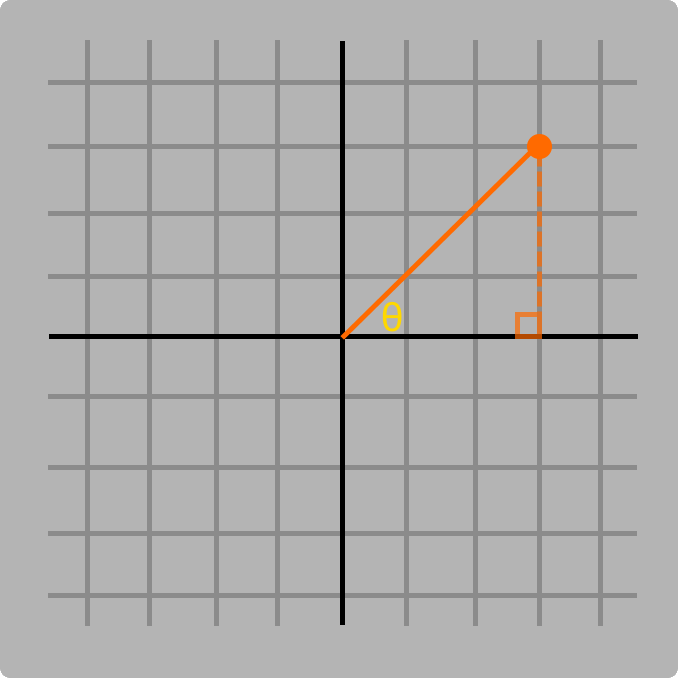
\includegraphics[scale=0.3]{Images/1.6.1.png}
    \end{figure}



    \begin{example}
        Convert $(x+1)^2 + (y-2)^2$ = 9 into polar coordinates.    
    \end{example}

    \begin{tbox}
        $x^2 + 2x + 1 + y^2 - 4y + 4$ = 9

        $r^2 + 2r\cos(\theta) - 4r\sin(\theta)$ = 4
    \end{tbox}

    \newpage



    \begin{definition}{Cylindrical Coordiantes}{14cm}
        While polar coordinates are the circular equivalent to $\mathbb{R}^2$,
        cylindrical
        
        coordinates are the circular equivalent to $\mathbb{R}^3$.
        
        {\color{lblue} Cylindrical coordinates} are expressed as
        $(r,\theta,z)$ where:

        \hspace{0.5cm}
        x = r cos($\theta$)
        \hspace{1cm}
        y = r sin($\theta$)
        \hspace{1cm}
        z = z
    \end{definition}

    \begin{figure}[h]
        \centering
        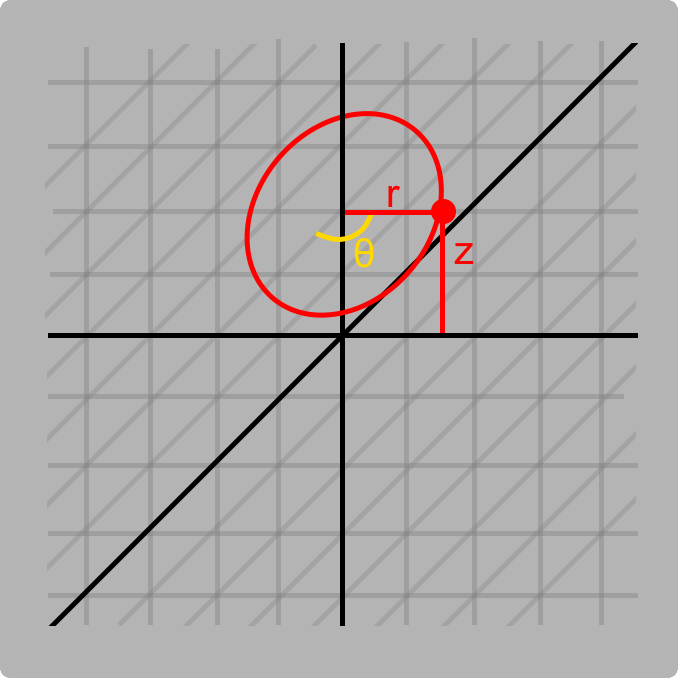
\includegraphics[scale=0.3]{Images/1.6.2.png}
    \end{figure}



    \begin{example}
        Convert z = 5r to rectangular coordinates.
    \end{example}

    \begin{tbox}
        z$^2$ = 25r$^2$
        \hspace{1cm}
        $\Rightarrow$
        \hspace{1cm}
        z$^2$ = 25($x^2+y^2$)
        \hspace{1cm}
        $\Rightarrow$
        \hspace{1cm}
        z = $5\sqrt{x^2+y^2}$
    \end{tbox}

    \vspace{0.5cm}



    \begin{definition}{Spherical Coordiantes}{14cm}
        Although way to express coordiantes in $\mathbb{R}^3$ is spherical
        coordiantes.

        {\color{lblue} Spherical coordinates} are expressed as
        $(p,\theta,\phi)$ where:

        \hspace{0.5cm}
        x = $p \sin(\phi) \cos(\theta)$
        \hspace{1cm}
        y = $p \sin(\phi) \sin(\theta)$
        \hspace{1cm}
        z = $p \cos(\phi)$

        where p = $r^2 + z^2$ = $x^2 + y^2 + z^2$ $\geq$ 0,
        $\theta$ $\in$ $[0,2\pi]$, and $\phi$ $\in$ $[0,\pi]$
    \end{definition}

    \begin{figure}[h]
        \centering
        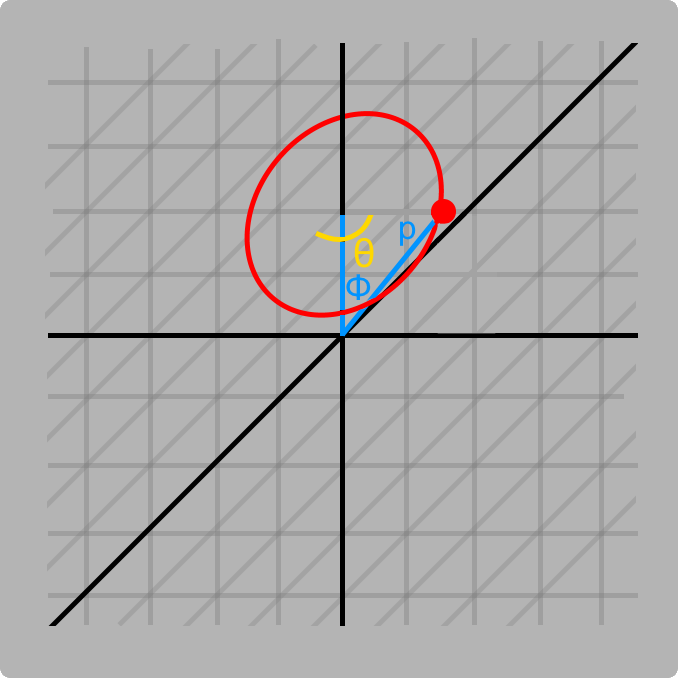
\includegraphics[scale=0.3]{Images/1.6.3.png}
    \end{figure}



    \begin{example}
        Convert z = 5r to spherical coordinates.
    \end{example}

    \begin{tbox}
        z = 5r
        \hspace{0.5cm}
        $\Rightarrow$
        \hspace{0.5cm}
        $\frac{r}{z}$ = $\frac{1}{5}$
        \hspace{0.5cm}
        $\Rightarrow$
        \hspace{0.5cm}
        tan($\phi$) = $\frac{1}{5}$
    \end{tbox}




